\documentclass[10pt, reqno]{amsart}
\setlength{\parindent}{0pt}
\usepackage{amssymb}
\usepackage{amscd}
\usepackage{verbatim,ifthen}
%\usepackage{libertine}
\usepackage{color}
\usepackage{latexsym}

\usepackage{setspace}
\onehalfspacing

\usepackage{graphicx}
\graphicspath{ {./images/} }

\usepackage{mathrsfs}
\usepackage{wrapfig}

\usepackage{pgfplots}
\usepackage{multicol}
\usepackage{array}
\newcolumntype{M}[1]{>{\centering\arraybackslash}m{#1}}
\def\heading#1{\centerline{\bf #1 }\vskip 12pt}
\newcommand\nextpage{\vfill\eject}
\usepackage[colorlinks, linkcolor=blue, citecolor=magenta, linktocpage]{hyperref}
%\addtolength{\textwidth}{80pt}
%\addtolength{\hoffset}{-40pt}
%\renewcommand{\baselinestretch}{1.2}

\addtocontents{toc}{\setcounter{tocdepth}{1}}

\usepackage[url=false, isbn=false, doi=false, eprint=false, citestyle=nature]{biblatex}
\addbibresource{library.bib}





\usepackage{graphicx,wrapfig,lipsum}
\usepackage{etoolbox}
\usepackage{marginnote}
%\usepackage{lipsum}
\makeatletter
\patchcmd{\@mn@margintest}{\@tempswafalse}{\@tempswatrue}{}{}
\patchcmd{\@mn@margintest}{\@tempswafalse}{\@tempswatrue}{}{}
\reversemarginpar 
\makeatother
\usepackage{scrextend}

\usepackage{titlesec}

\titleformat{\section}
  {\Large\scshape}{\thesection}{1em}{}
\usepackage[margin=1in]{geometry}





\title{Evaluating the Ruggedness of Protein Fitness Landscapes}

\author{Mahakaran Sandhu, Adam Mater, Colin Jackson* }

\begin{document}

\maketitle

\begin{abstract}
    This is the abstract.
\end{abstract}



\section{Introduction}

Relevance/importance \\
Similar work \\
Aims \\
Outline\\

\clearpage
\section{Results}
\subsection{Explanation of the metrics.}
\begin{enumerate}
    \item Number of local maxima.
    \item Random walk methods
    \item Roughness to slope ratio
    \item Fourier expansion
\end{enumerate}


\subsection{Validation on Synthetic Landscapes.}

Explanation of synthetic landscapes used. 

\subsubsection{Accounting for sequence length.}

In real-world empirical datasets there is a need to be able to measure ruggedness for different lengths $N$ and amino acid/nucleotide alphabets $A$. Szendro and colleagues \supercite{Szendro2013} effectively circumvented this problem for binary alleles $A$ and few $N$ by calculating ruggedness metrics systematically over subgraphs of sequence space; empirical protein datasets have far larger values of $|A|$ and $N$, and this approach quickly becomes computationally intractable (see SI \hyperref[subgraph problem]{Subgraph Problem}). Therefore, we sought alternative approaches. The idiosyncrasies of the individual metrics called for tailored normalisation approaches; we address each individually below.\\


\textbf{Number of local maxima.} $N_{max}$ is a global measure of a landscape's ruggedness that is dependent not only on ruggedness but also $N$ and $A$ \supercite{Szendro2013, Kauffman1993}. As $N$ and $A$ increase, $N_{max}$ also increases, despite constant ruggedness (proof?/ref? see SI). The maximum number of $N_{max}$ is given by $\max (N_{max}) = \frac{|A|^N}{N+1}$ (see SI \hyperref[SI properties]{Properties of fitness landscapes}). If we assume that underlying ruggedness is constant for increasing $N, A$, then a straightforward normalisation strategy is to divide the calculated $N_{max}$ by $\max (N_{max})$ given $N,A$. We tested this strategy for $NK$ and RMF \supercite{Neidhart2014} landscapes. \\














\textbf{Random walk methods.} These should be really easy because of ergodic theorem etc, and because this is a local property \\

 \textbf{r/s ratio.} This will be hard\\

 \textbf{Fourier.} this may also be hard (although when we distill down to 'percent contribution' of higher order terms it doesn't really seem like it should be that much more difficult. \supercite{Neidhart2013}





\subsubsection{Accounting for fitness scale}
\subsubsection{Accounting for non-linearity}
\subsubsection{Accounting for incomplete datasets/sampling}


\subsection{Validation on Real Datasets}

\section{Discussion}

Discussion of properties and limitations of the metrics \\
Discussion of other metrics and future work\\
Discussion of surrounding literature (e.g. global epistasis, minimum epistasis etc) \\
Implications for evolution and directed evolution\\
Implications for ML \\



The assumption that ruggedness is an intensive property of fitness landscapes ( i.e. ruggedness is constant for arbitrary partitions of the landscape) is valid only in the case of statistically isotropic landscapes; in anisotropic landscapes, ruggedness may differ in different regions of the landscape. In an anistotropic landscape, we would expect the distribution of $N_{max}$) to also be anisotropic. Using $N_{max}$ it may therefore be possible to map out regions of high ruggedness, and use dimensionality reduction techniques (such as those proposed by McLandlish Evolution. 2011 Jun; 65(6): 1544–1558.) to visualise the distribution of ruggedness in an empirical landscape.



\section{Methods}

\section{Supporting Information}

\subsubsection{Ruggedness itself}




\subsection{Properties of fitness landscapes}

\subsubsection*{ Property 1. ($\max N_{max}$ as a function of $A, N$)} 
The probability $P_m$ that a given sequence is a local maximum is the probability that it has higher rank-order than any of its $Q$ one-mutant neighbours \supercite{Kauffman1993, Kauffman1987, Rosenberg2005}

\begin{equation}
    P_m= \frac{1}{Q+1} = \frac{1}{N(|A|-1)+1} 
\end{equation}

It then follows that the maximum possible number of local optima is given by

\begin{equation}
    \max N_{max} =  \frac{|A|^N}{N(|A|-1)+1}
\end{equation}

where $|A|^N$ is the expression for the size of the sequence space $|S|$. This result is applicable to any HoC landscape (is it? ref? proof?). In the HoC case, we assume that underlying ruggedness is maximal, even though the dimensionality of the space changes with $A$ and $N$; how $N_{max}$ changes with $K$ is mathematically complex (cite cite cite). While we do not offer a proof for this conjecture, we appeal to intuition (below). 

\subsubsection*{Statistical isotropy, homogeneity, ruggedness and $N_{max}$.}

Suppose that a HoC landscape is statistically isotropic and homogeneous. This implies that any equally-sized connected subgraph/partition $P \subseteq \mathcal{G}(V,E) $ of the fitness graph will have the same expectation of local maxima, $\mathbb{E}(N_{max})$, i.e. the density of local maxima is constant throughout the landscape, $\rho(N_{max})$. This further implies that the naive probability that any vertex $V$ is a local maximum is identical throughout the landscape. This intuition follows from Property 1. We might venture to say that the \textit{ruggedness} with respect to $N_{max}$ of the landscape is uniform throughout the landscape. (One caveat is that even though the landscape is isotropic in terms of $N_{max}$, the magnitude difference in different regions of the landscapes may not be -- this may be evaluated by taking the second-order calculation of the average magnitude difference of local maxima with respect to 1-mutant neighbours and then taking the distribution of the calculated quantity -- a complex distribution would indicate anisotropy). \\

However, it is unclear how we might think about comparing ruggedness in differently-sized landscapes, specifically, different $|A|$ and $N$. Supposing statistical isotropy and homogeneity, we would have to scale the partition $P \subseteq \mathcal{G}(V,E)$ by some factor that takes into account the dimensionality of the space. From a naive graph-theoretic perspective, if the density of $N_{max}$ and the degree distribution is constant, adding new nodes to a graph ought not to change $\rho(N_{max})$. The total number of maxima will increase, but we can easily obtain $\rho(N_{max})$ by normalising for the increased number of nodes. This simplistic case, however, does not hold in a Hamming graph, where the degree distribution changes as well as the number of nodes. Thus, normalising for constant $\rho(N_{max})$ must take into account the changed degree distribution. In particular, the probability that any given vertex is a local maxima changes as $ \frac{1}{N(|A|-1)+1} $. Therefore, as $N$ and $|A|$ increase, the probability decreases as a linear function of both $N$ and $|A|$. However, the total number of maxima increases dramatically as $|A|^N$. Therefore, to satisfactorily compare ruggedness between different sized landscapes, it seems necessary to correct for the probability decrease, as well as the dramatic increase in space size. This result allows us to compute $\rho(N_{max})$ for different sized HoC landscapes. To compare ruggedness values for non-HoC landscpaes (i.e. most real landscapes), we calculate the ratio $N_{max}^{real}/N_{max}^{HoC}$, giving us a proxy for ruggedness as a fraction of total possible ruggedness with respect to $N_{max}$ given $|A|$ and $N$; through this relation, we can compare ratios for differently-sized landscapes because we know how HoC $N_{max}$ can be compared between differently-sized landscapes. \\

Is the above argument valid? Ask J. Krug? \\





\begin{figure}[h]
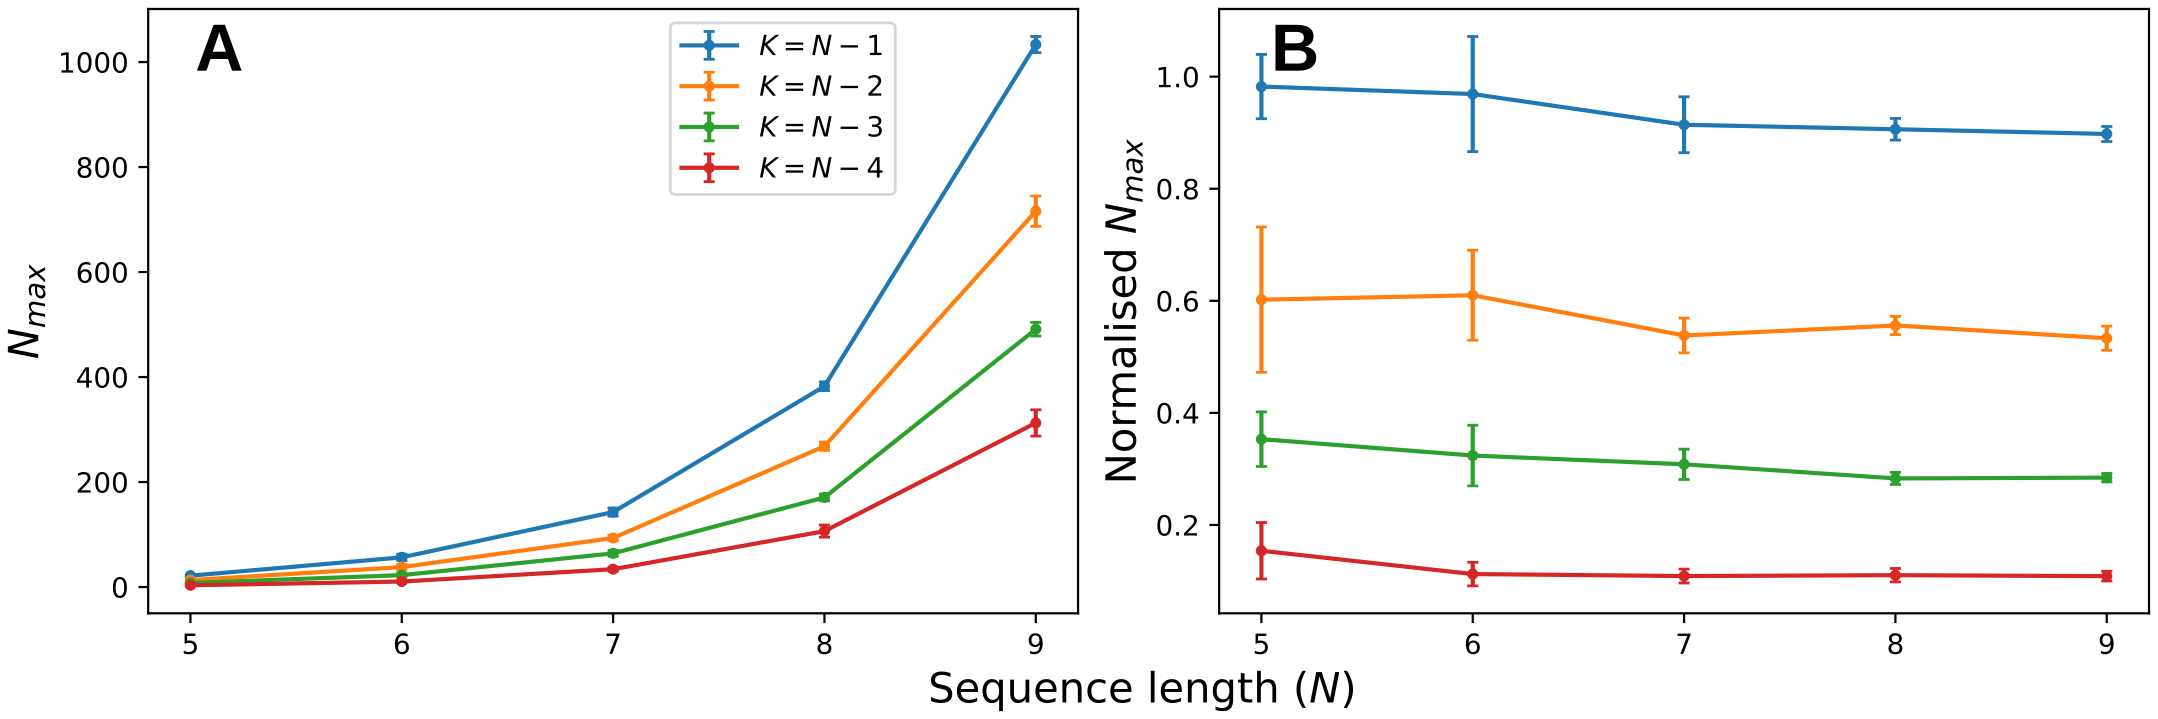
\includegraphics[scale=0.6]{images/seq_len_vs_nmax_figure.png}
\caption{\textbf{(A)} $N_{max}$ at increasing sequence lengths $N$ and different $K$ values (legend); $K$ values are defined in terms of subtraction from $N$ to give roughly similar ruggedness $N/K$ values; $K = N-1$ gives the maximally-ruggedn HoC case. \textbf{(B)} Normalised $N_{max}$ values with ruggedness correction. See Methods for detailed normalised procedure. Differences within $K$ values are insignificant; between $K$ values, differences are significant. We note that there is a non-linear relationship between increasing $K$ and normalised $N_{max}$, the exact nature of of which is outside the scope of this work and needs to be checked (might have to use a different model to get around this). \textbf{(C)} This will be un-normalised changes in Nmax as alphabet increases. \textbf{(D)} This will be the normalised version.}

\end{figure}






We further note that $N_{max}$ as a metric loses information regarding the isotropy or lack thereof of the fitness landscape; it assumes that the landscape is isotropic. To circumvent this limitation, we have implemented the average height of fitness maxima. 













\subsection{Subgraph Problem}

\subsubsection*{Definition 1. (Sequence space subgraphs)} A subgraph of size $m < L$ is the set of all combinations of the alleles at $m$ of the $L$ loci at a fixed state of the remaining $L-m$ `background' loci. There are ${L \choose m}$ subsets of $m$ loci and (for the bi-allelic case) $2^{L-m}$ backgrounds; and thus the total number of subgraphs is $2^{(L-m)}{L \choose m}$. If there are $A$ possible alleles, then there are $A^{L-m}$ backgrounds, and the total number of subgraphs is $A^{(L-m)}{L \choose m}$; each subgraph will have $A^m$ sequences, for a total of $A^m A^{(L-m)}{L \choose m} = A^L$ sequences (Krug, J. and de Visser, JAG, personal communication). \\



\subsubsection*{Problem} Consider a protein of length $N$, where $N$ is nontrivially large (e.g. $N > 100$). For this example, let $N=100$. While the sequence space $S$ has size $A^N$, we assume here that we are dealing with an incomplete experimental dataset $D \in S$. Let the the structure of mutations in $D$ be random, i.e. any given position $p_i \in N$ will be found mutated at some sequence $d \in D$. We desire to generate a set of subgraphs $\Sigma$ with size $m = 4$ from the experimental dataset $D$. \\


\subsubsection*{Solution 1. (Non-heuristic sorting algorithm)}
Generating all possible subgraphs $\Sigma$ requires enumerating a ruleset for membership in any given subgraph $\sigma \in \Sigma$, and then performing a search through the dataset $D$ for sequences $d$ that fulfill the membership ruleset for a given $\sigma \in \Sigma$. In our example, the size of $\Sigma$ is  $A^{(L-m)}{L \choose m} = 20^{(100-4)}{100 \choose 4} = 20^{96} \times 3921225$ (here $L=N$), which is clearly intractable, even if only generating empty subgraphs containing only the ruleset. Note that if this program were run on an incomplete experimental dataset $D$, many of the subgraphs would be empty. \\


\subsubsection*{Solution 2. (Heuristic sorting algorithm)} 

Generating an incomplete subgraph set $\Sigma^*$ with valid but incomplete subgraphs $\sigma ^*$ can be acheived by enumerating an incomplete set of rulesets $r^* \in R$ that correspond to $\sigma \in \Sigma$, and then performing a search through the dataset $D$ for sequences $d$ that fulfill some $r \in r^*$. This is a tractable program when $\text{size}(r^*) << \text{size}(R)$.  




\printbibliography





\end{document}
